\section{紧致性}
\label{sec:metric-compactness}

实轴上的闭区间有两条重要性质：其中的数列总有收敛子列，连续函数在其上取得最大值和最小值。开区间$(0,1)$和整条实轴都没有这些性质。本节寻找一般度量空间中与“闭区间”对应的条件。它的核心是有限性：无论精度多高，集合都能由有限个小球控制。我们先从覆盖的角度提出这一要求，再把它与收敛子列、完备性联系起来。

\subsection{有界集与全有界集}
\label{sec:metric-totally-bounded}

“集合不太大”最直接的说法是：它能装进一个有限半径的球中。

\begin{definition}[有界集]
\label{def:metric-bounded}
若存在$a\in X$与$R<\infty$使$A\subseteq B(a,R)$，就称$A\subseteq X$是\term{有界}（bounded）的。非空集合$A$的\term{直径}（diameter）定义为$\operatorname{diam}A=\sup_{x,y\in A}d(x,y)$。
\end{definition}

两种说法等价：若$A\subseteq B(a,R)$，三角不等式给出$d(x,y)\leq d(x,a)+d(a,y)<2R$，所以$\operatorname{diam}A\leq2R$；反过来，若$\operatorname{diam}A<\infty$，任取$a\in A$，则$A\subseteq B(a,\operatorname{diam}A+1)$。

有界只控制集合的总体范围，不控制集合的内部能否在细尺度下被少量信息描述。离散度量下的无限集合$X$直径为$1$，因而有界；但用半径$1/2$的球覆盖它时，每个球只含一个点，需要无限多个球。下面的定义要求每个尺度都只需有限个球。

\begin{definition}[全有界与$\varepsilon$网]
\label{def:metric-totally-bounded}
设$A\subseteq X$，$\varepsilon>0$。若有限集$\{a_1,\dots,a_k\}\subseteq A$满足$A\subseteq\bigcup_{i=1}^kB(a_i,\varepsilon)$，就称它是$A$的一个有限$\varepsilon$网（finite $\varepsilon$-net），不指明精度时简称\term{有限网}。若对每个$\varepsilon>0$，$A$都有有限$\varepsilon$网，就称$A$是\term{全有界}（totally bounded）的。
\end{definition}

$\varepsilon$网中的点是在精度$\varepsilon$下代表$A$的有限个样本：$A$中每一点都与某个代表点相距不到$\varepsilon$。代表点的个数和位置可以随$\varepsilon$改变，精度越高通常需要越多代表点，但对每个精度都必须是有限个。图~\ref{fig:metric-epsilon-net}画出了同一个集合在两种精度下的网。

\begin{figure}[!htbp]
  \centering
  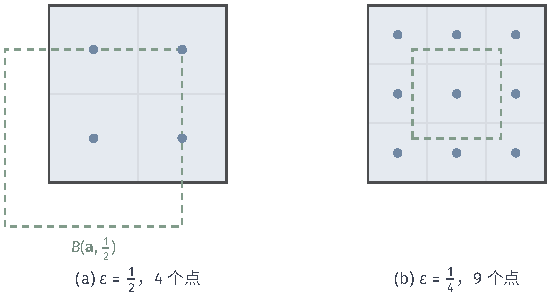
\includegraphics[width=93.169mm]{figures/02-abstract-mathematics/01-metric-and-measure/tikz/c1-epsilon-net/figure.pdf}
  \caption{正方形$[0,1]^2$在$d_\infty$下的有限$\varepsilon$网。把正方形等分为小格，蓝点取在各小格中心，小格中的点与该格中心的$d_\infty$距离至多为半个格宽。(a) $\varepsilon=1/2$时用$4$个点$\bigl((2i-1)/4,(2j-1)/4\bigr)$，格内距离至多$1/4<1/2$；虚线正方形是其中一个球$B(\bm a,1/2)$。(b) $\varepsilon=1/4$时用$9$个点$\bigl((2i-1)/6,(2j-1)/6\bigr)$，格内距离至多$1/6<1/4$。精度提高时代表点增多，但始终是有限个。}
  \label{fig:metric-epsilon-net}
\end{figure}

\paragraph{全有界推出有界与可分}
全有界比有界强。取一个有限$1$网$\{a_1,\dots,a_k\}$，任意$x,y\in A$分别落在某个$B(a_i,1)$与$B(a_j,1)$中，于是$d(x,y)<2+\max_{i,j}d(a_i,a_j)$，$A$有界。全有界还推出$A$（作为子空间）可分：对每个$n$取一个有限$1/n$网$F_n$，令$D=\bigcup_nF_n$，它是可数个有限集的并，因而可数。对任意$x\in A$与$r>0$，取$n>1/r$，$F_n$中有一点与$x$相距小于$1/n<r$，所以$D$在$A$中稠密。

\paragraph{三个要求的区别}
两个反例说明这些蕴含不能反过来。无限离散空间有界，但对$\varepsilon=1/2$没有有限网，因而不全有界。通常距离下的$\mathbb R$可分（有可数稠密集$\mathbb Q$），却无界，也就不全有界。有界控制总体范围，可分要求一套可数代表服务于所有精度，全有界则要求每个精度下只需有限个代表；三者各自约束不同的东西。

\subsection{开覆盖与紧致集}
\label{sec:metric-open-cover}

全有界允许我们为每个精度挑选最方便的一组球。有些论证中，球不是我们挑的，而是别人给定的一族开集，例如“每一点各自有一个让函数变化不大的邻域”。紧致性要求：无论给定怎样的开覆盖，都能从中选出有限个成员完成覆盖。

\begin{definition}[紧致集]
\label{def:metric-compact}
若一族开集$\{U_\alpha\}_{\alpha\in I}$满足$X=\bigcup_{\alpha\in I}U_\alpha$，就称它是$X$的一个\term{开覆盖}（open cover）。若$X$的每个开覆盖都有有限子族$U_{\alpha_1},\dots,U_{\alpha_k}$仍覆盖$X$，就称度量空间$X$是\term{紧致}（compact）的。若子集$K\subseteq X$配备子空间度量后是紧致的，就称$K$是紧致集（或紧集）。
\end{definition}

由引理~\ref{lem:metric-relative-open}，$K$中的开集都形如$K\cap V$，$V$在$X$中开。所以$K$紧致，等价于：每一族满足$K\subseteq\bigcup_\alpha V_\alpha$的$X$中的开集都有有限子族仍覆盖$K$。定义中的“有限子覆盖”必须从给定的覆盖中挑选，不能另换一组更方便的开集；正是这一点使紧致性比全有界强。

\paragraph{紧致集全有界且闭}
把全部半径为$\varepsilon$的球$\{B_K(x,\varepsilon):x\in K\}$作为开覆盖代入定义，有限子覆盖的中心就是一个有限$\varepsilon$网，所以紧致集全有界。紧致集还在任何环境空间中都是闭集。设$x\in X\setminus K$。对每个$y\in K$，令$r_y=d(x,y)/2>0$，开球$B(y,r_y)$覆盖$K$，取有限子覆盖$B(y_1,r_{y_1}),\dots,B(y_k,r_{y_k})$，令$r=\min_ir_{y_i}>0$。若$z\in B(x,r)\cap B(y_i,r_{y_i})$，则$d(x,y_i)\leq d(x,z)+d(z,y_i)<r+r_{y_i}\leq2r_{y_i}=d(x,y_i)$，矛盾；所以$B(x,r)$与$K$不交。外点都有避开$K$的球，$K$闭。

\begin{example}[全有界而不紧致]
\label{ex:metric-open-interval-cover}
$(0,1)$在通常距离下全有界：对$\varepsilon>0$，取有限个间距小于$\varepsilon$的点即可。但$(0,1)$不紧致。令$U_n=(1/n,1)$（$n\geq2$），每一点$x\in(0,1)$在$n>1/x$时属于$U_n$，所以$\{U_n\}$覆盖$(0,1)$。任取有限个$U_{n_1},\dots,U_{n_k}$，它们的并是$(1/N,1)$，其中$N=\max_in_i$，它漏掉了$(0,1/N]$中的点。图~\ref{fig:metric-open-cover-interval}画出了这个覆盖。用有限个小球覆盖$(0,1)$并不困难，难点在于这个给定覆盖的成员越来越靠近$0$而永远不包含它附近的全部点。
\end{example}

\begin{figure}[!htbp]
  \centering
  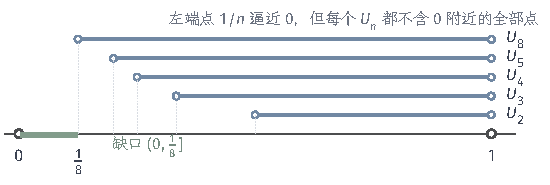
\includegraphics[width=93.105mm]{figures/02-abstract-mathematics/01-metric-and-measure/tikz/c1-open-cover/figure.pdf}
  \caption{开区间$(0,1)$的一个没有有限子覆盖的开覆盖。各条蓝色线段是$U_n=(1/n,1)$，$n=2,3,4,5,8$，它们的左端点$1/n$逐渐逼近$0$却不到达$0$；任取有限个成员，并集是某个$(1/N,1)$，在$0$附近留下绿色标出的缺口$(0,1/N]$。}
  \label{fig:metric-open-cover-interval}
\end{figure}

无限离散空间提供了另一类反例：它闭（作为全空间）且有界，但全部单点开球$\{\{x\}\}$组成开覆盖，任何有限子族只覆盖有限个点，所以不紧致。在一般度量空间中，“闭且有界”不足以推出紧致。

\subsection{紧致性的序列刻画}
\label{sec:metric-sequential-compactness}

闭区间上“数列有收敛子列”的性质也可以作为紧致性的定义。在度量空间中，它与开覆盖的定义等价。

\begin{definition}[序列紧致]
\label{def:metric-sequentially-compact}
若$K$中的每个点列都有在$K$中收敛的子列，就称$K\subseteq X$是\term{序列紧致}（sequentially compact）的。
\end{definition}

\begin{theorem}[紧致性的序列刻画]
\label{thm:metric-compact-sequential}
度量空间的子集$K$紧致，当且仅当它序列紧致。
\end{theorem}

\begin{proof}
\emph{紧致推出序列紧致。}设$K$紧致，$(x_n)$是$K$中的点列。先证明存在$y\in K$，使每个球$B(y,r)$都含有点列中下标无限多的项。若不然，每个$y\in K$都有半径$r_y>0$，使$B(y,r_y)$只含有限个下标$n$的$x_n$。这些球覆盖$K$，取有限子覆盖$B(y_1,r_{y_1}),\dots,B(y_k,r_{y_k})$。每个$x_n$都在其中某个球内，而每个球只容纳有限个下标，于是下标总数有限，与点列有无限多个下标矛盾。

再由这样的$y$构造收敛子列。取$n_1$使$x_{n_1}\in B(y,1)$；设已取$n_1<\cdots<n_k$，由于$B(y,1/(k+1))$含有下标无限多的项，可以取$n_{k+1}>n_k$使$x_{n_{k+1}}\in B(y,1/(k+1))$。于是$d(x_{n_k},y)<1/k\to0$，子列在$K$中收敛到$y$。

\emph{序列紧致推出紧致。}设$K$序列紧致。第一步证明$K$全有界。若对某个$\varepsilon>0$没有有限$\varepsilon$网，任取$x_1\in K$；设已取$x_1,\dots,x_n$，它们不是$\varepsilon$网，所以有$x_{n+1}\in K$不在$\bigcup_{i\leq n}B(x_i,\varepsilon)$中。所得点列两两距离至少为$\varepsilon$，它的任何子列都不是柯西列，也就不收敛，与序列紧致矛盾。

第二步证明：对$K$的任意开覆盖$\{U_\alpha\}$，存在$\delta>0$，使每个$x\in K$的球$B_K(x,\delta)$都包含于某个$U_\alpha$。若不然，对每个$n$都有$x_n\in K$，使$B_K(x_n,1/n)$不包含于任何$U_\alpha$。取子列$x_{n_k}\to x\in K$。$x$属于某个$U_\beta$，又因$U_\beta$在$K$中开，有$r>0$使$B_K(x,r)\subseteq U_\beta$。取$k$充分大，使$d(x_{n_k},x)<r/2$且$1/n_k<r/2$。对$z\in B_K(x_{n_k},1/n_k)$有$d(z,x)<1/n_k+r/2<r$，所以$B_K(x_{n_k},1/n_k)\subseteq B_K(x,r)\subseteq U_\beta$，矛盾。

第三步完成覆盖。由第一步取有限$\delta$网$\{a_1,\dots,a_m\}$，由第二步每个$B_K(a_i,\delta)$包含于某个$U_{\alpha_i}$。这些球覆盖$K$，所以$U_{\alpha_1},\dots,U_{\alpha_m}$覆盖$K$。
\end{proof}

第二步得到的$\delta$称为该覆盖的\term{Lebesgue数}（Lebesgue number）：只要观察范围小于$\delta$，就不必担心跨越覆盖成员的边界。整个证明反复使用距离：用$1/k$半径的球选子列，用两两距离判断子列不是柯西列，用三角不等式比较两个球。对没有度量的一般拓扑空间，紧致与序列紧致可以不等价，本章不讨论那种情形。

\subsection{完备与全有界判据}
\label{sec:metric-complete-totally-bounded}

开覆盖条件难以直接验证。下面的判据把紧致性拆成两个分别容易检查的条件：完备性保证柯西列有极限，全有界性保证能抽出柯西子列。

\begin{theorem}[紧致的完备全有界判据]
\label{thm:metric-compact-complete-tb}
度量空间$K$紧致，当且仅当$K$完备且全有界。
\end{theorem}

\begin{proof}
设$K$紧致。全有界已在第~\ref{sec:metric-open-cover}小节证明。对完备性，设$(x_n)$是$K$中的柯西列。由定理~\ref{thm:metric-compact-sequential}，有子列$x_{n_k}\to x\in K$。对$\varepsilon>0$取$N$使$m,n\geq N$时$d(x_m,x_n)<\varepsilon/2$，再取$k$使$n_k\geq N$且$d(x_{n_k},x)<\varepsilon/2$，则$n\geq N$时$d(x_n,x)\leq d(x_n,x_{n_k})+d(x_{n_k},x)<\varepsilon$。所以整个柯西列收敛到$x$。

反过来，设$K$完备且全有界，$(x_n)$是$K$中的点列。用有限个半径$1$的球覆盖$K$，其中至少有一个球含有下标无限多的项，记这些下标的集合为$I_1$。再用有限个半径$1/2$的球覆盖$K$，其中某个球含有$\{x_n:n\in I_1\}$中下标无限多的项，记这些下标为$I_2\subseteq I_1$。如此继续，得到无限下标集$I_1\supseteq I_2\supseteq\cdots$，其中$I_j$对应的项都落在同一个半径$1/j$的球中。取$n_1\in I_1$，再依次取$n_j\in I_j$且$n_j>n_{j-1}$。当$k,l\geq j$时，$x_{n_k}$与$x_{n_l}$都属于$I_j$所对应的球，故$d(x_{n_k},x_{n_l})<2/j$。子列$(x_{n_j})$是柯西列，由完备性在$K$中收敛。于是$K$序列紧致，由定理~\ref{thm:metric-compact-sequential}，$K$紧致。
\end{proof}

用这一判据重看前面的例子：$(0,1)$全有界但不完备，无限离散空间完备（其中的柯西列从某项起为常数）但不全有界，二者都不紧致；$[0,1]$完备且全有界，因而紧致。

\paragraph{欧氏空间中的闭有界集}
在$\mathbb R^d$中，有界与全有界一致，于是判据简化为熟悉的形式。

\begin{theorem}[欧氏空间的闭有界判据]
\label{thm:metric-heine-borel}
在$(\mathbb R^d,d_2)$中，子集$K$紧致当且仅当它闭且有界。
\end{theorem}

\begin{proof}
紧致集闭且有界已在第~\ref{sec:metric-open-cover}小节证明。反过来，设$K$闭且有界，则存在$M$使$K\subseteq[-M,M]^d$。$\mathbb R^d$完备而$K$闭，由定理~\ref{thm:metric-complete-closed}，$K$完备。对全有界，给定$\varepsilon>0$，取正整数$s$使边长$h=2M/s<\varepsilon/\sqrt d$，把$[-M,M]^d$等分为$s^d$个边长为$h$的闭小立方体。每个小立方体中两点的欧氏距离至多为$h\sqrt d<\varepsilon$。在每个与$K$相交的小立方体中取一点$a_Q\in K$，得到至多$s^d$个点；$K$中任一点所在的小立方体也含有对应的$a_Q$，二者距离小于$\varepsilon$。所以这些点组成$K$的有限$\varepsilon$网。由定理~\ref{thm:metric-compact-complete-tb}，$K$紧致。
\end{proof}

证明中有限维出现在网格的计数$s^d$上：维数固定时，网格点数有限。特别地，$\mathbb R$中的闭区间$[a,b]$紧致，闭区间上数列有收敛子列的性质成为定理~\ref{thm:metric-compact-sequential}的特例。在一般度量空间（包括后面要讨论的函数空间）中，闭有界集不一定紧致，必须回到“完备且全有界”来判断。
